\documentclass[12pt]{ctexart}
    %%% Document Settings %%%%
%\usepackage[utf8]{inputenc}

\usepackage[
    twoside,
    top=1in,
    bottom=0.75in,
    inner=0.5in,
    outer=0.5in,
]{geometry}
\pagestyle{myheadings}
\usepackage{minted}
\usepackage[dvipsnames,svgnames]{xcolor}

%%%% Additional Commands to Load %%%%
\usepackage{tcolorbox}
\tcbuselibrary{skins}
\tcbuselibrary{minted}
\usemintedstyle{lovelace}
%\usepackage{minted}
\usepackage{color}
\usepackage{tikz}
\usetikzlibrary{calc}
\usepackage{tabularx,colortbl}
\usepackage{amsfonts,amsmath,amssymb}
\usepackage{titling}
\usepackage{mathrsfs}
\usepackage{calc}
\usepackage{subcaption}

\usepackage{listings}
%\usepackage{newtxtext}
\usepackage[strict]{changepage} 
\usepackage{framed}
\definecolor{formalshade}{rgb}{0.95,0.95,1}
\usepackage{float}

%%%% Commands to Define Homework Boxes %%%%
%%%% Box Definition %%%%
\newtcolorbox{prob}[1]{
% Set box style
    sidebyside,
    sidebyside align=top,
% Dimensions and layout
    width=\textwidth,
    toptitle=2.5pt,
    bottomtitle=2.5pt,
    righthand width=0.20\textwidth,
% Coloring
    colbacktitle=gray!30,
    coltitle=black,
    colback=white,
    colframe=black,
% Title formatting
    title={
        #1 \hfill Grade:\phantom{WWWW}
    },
    fonttitle=\large\bfseries
}

%%%% Environment Definition %%%%
\newenvironment{problem}[1]{
    \begin{prob}{#1}
}
{
    \tcblower
    \centering
    \textit{\scriptsize\bfseries Faculty Comments}
    \vspace{\baselineskip}
    \end{prob}
}

\newenvironment{formal}{%
\def\FrameCommand{%
\hspace{1pt}%
{\color{DarkBlue}\vrule width 2pt}%
{\color{formalshade}\vrule width 4pt}%
\colorbox{formalshade}%
}%
\MakeFramed{\advance\hsize-\width\FrameRestore}%
\noindent\hspace{-4.55pt}% disable indenting first paragraph
\begin{adjustwidth}{}{7pt}%
\vspace{2pt}\vspace{2pt}%
}
{%
\vspace{2pt}\end{adjustwidth}\endMakeFramed%
}

    \title{特殊方程作业1}
    \author{地物2201班\ 杨曜堃}
    \date{\today}
%%% document
\begin{document}

% Format Running Header
    \markboth{\theauthor}{\thetitle}
    \maketitle
    \begin{description}
        \item[问题1] 设弦的两端固定与$x=0$及$x=L$,弦的初始位移如图所示,初速度为0,又没有外力作用,试写出相应的定解问题。
    \end{description}

    \begin{center}
        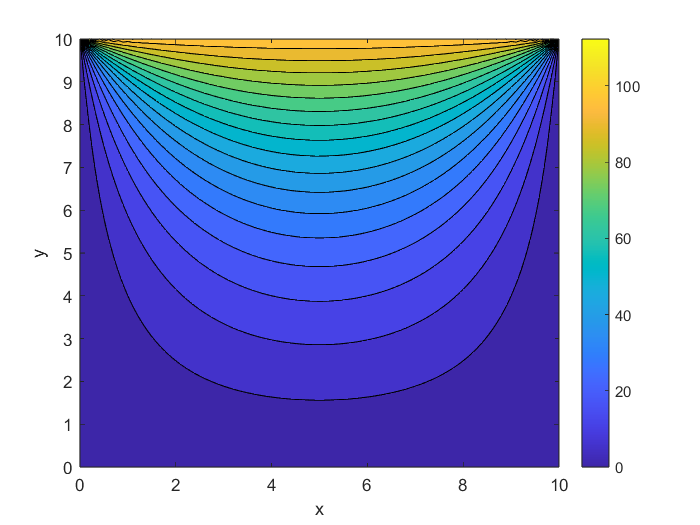
\includegraphics[width=16cm]{fig1.png}
    \end{center}
    
    \begin{problem}{问题\#1}
        已知弦的振动满足一维波动方程(忽略重力)
        $$
        \dfrac{\partial^2u}{\partial t^2}=a^2\dfrac{\partial^2u}{\partial x^2}
        $$
        由初始位移可知定解问题的初始条件
        $$
        u(x,t)|_{t=0}=
            \begin{cases}
                \dfrac{h}{c}x, & \quad 0\leqslant x\leqslant c\\
                \dfrac{h}{c-L}x+\dfrac{hL}{L-c}, & \quad c<x\leqslant L
            \end{cases} 
        $$
        由于弦的两端固定、初速度为0、没有外力作用,因此采用Dirichlet边界条件
        $$
            u(x,t)|_{x=0}=u(x,t)|_{x=L}=0
        $$
        定解问题可以描述为
        $$
            \begin{cases}
                \dfrac{\partial^2u}{\partial t^2}=a^2\dfrac{\partial^2u}{\partial x^2},&\quad 0<x<L,t>0\\
                u|_{x=0}=0,u|_{x=L}=0,&\quad t\geqslant 0\\
                u|_{t=0}=\varphi(x)\\,\dfrac{\partial u}{\partial t}|_{t=0}=0,&\quad 0\leqslant x\leqslant L
            \end{cases}
        $$
        其中
        $$
        \varphi(x)=
            \begin{cases}
                \dfrac{h}{c}x, & \quad 0\leqslant x\leqslant c\\
                \dfrac{h}{c-L}x+\dfrac{hL}{L-c}, & \quad c<x\leqslant L
            \end{cases} 
        $$
    \end{problem}
\end{document}